% Created 2015-02-20 Пт 06:18
\documentclass[presentation]{beamer}


%%% Packages.

\usepackage[utf8]{inputenc}
\usepackage[T1]{fontenc}
\usepackage{fixltx2e}
\usepackage{graphicx}
\usepackage{longtable}
\usepackage{float}
\usepackage{wrapfig}
\usepackage{rotating}
\usepackage[normalem]{ulem}
\usepackage{amsmath, amssymb}
\usepackage{textcomp}
\usepackage{marvosym}
\usepackage{wasysym}
\usepackage{hyperref}
\tolerance=1000
\usepackage[english, russian]{babel}
\usepackage[labelformat=empty]{caption}
\usepackage{subcaption}
\usepackage{listings}
\usepackage{color}
\let\Cross\relax
\let\Square\relax
\usepackage{bbding}


%%%

\graphicspath{{graphics/}}

\usetheme[height=20pt]{Rochester}


%%% Title.

\author{Артём Попцов}
\date{2015-10-24}

\title{Введение в системы управления версиями}

\begin{document}

\maketitle


%%% TOC.

\begin{frame}{Содержание}
  \setcounter{tocdepth}{1}
  \tableofcontents
\end{frame}


%%%

\section{Задачи, решаемые системами управления версиями}

\subsection{Организация работы}

\begin{frame}{Организация работы}
  \begin{itemize}
  \item Начало работы
    \begin{itemize}
    \item курсовая.tex
    \end{itemize}
  \item Прошла неделя
    \begin{itemize}
    \item курсовая.tex, курсовая.tex.bak
    \end{itemize}
  \item Ещё некоторое время спустя
    \begin{itemize}
    \item курсовая.tex, курсовая.tex.bak, курсовая-old.tex
    \end{itemize}
  \item Показали преподавателю
    \begin{itemize}
    \item курсовая.tex, курсовая.tex.bak, курсовая-old.tex,
      курсовая-new.tex
    \end{itemize}
  \item Внесли изменения
    \begin{itemize}
    \item курсовая.tex, курсовая.tex.bak, курсовая-old.tex,
      курсовая-old2.tex, курсовая-final.tex
    \end{itemize}
  \item \ldots{}
  \end{itemize}
\end{frame}

\begin{frame}{В ходе работы возникают вопросы\ldots{}}
  \begin{itemize}
  \item Какая версия последняя (актуальная)?
  \item Где находится актуальная версия?  Она на флэшке?
  \item В чём различия между старой и новой версией?
  \item Я ничего не помню.  Что я делал вчера?
  \end{itemize}
\end{frame}

\begin{frame}{В ходе работы возникают вопросы\ldots{}}
  \begin{columns}
    \begin{column}{0.6\textwidth}
      \huge{\textbf{Ой!}  Я случайно перезаписал новую версию старой.\newline
        Что делать?..}
    \end{column}
    \begin{column}{0.4\textwidth}
      \begin{figure}[htb]
        \centering
        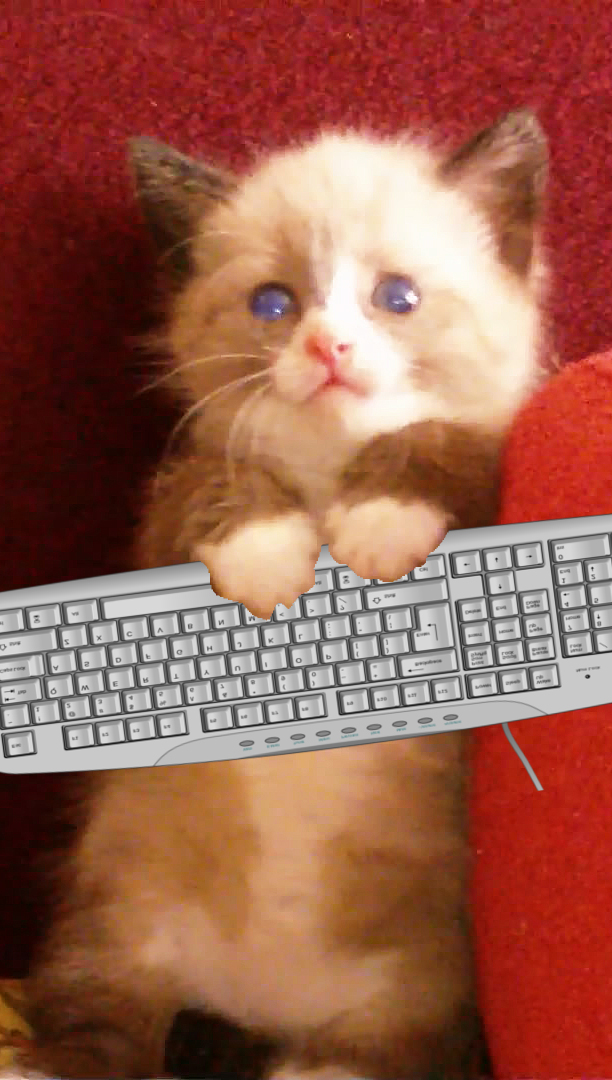
\includegraphics[width=1\textwidth]{chizhik-with-keyboard}
      \end{figure}
      \end{column}
  \end{columns}
\end{frame}


%%%

\section{Виды систем управления версий}

\subsection{Я должен использовать систему управления версиями!}
\begin{frame}{Я должен использовать систему управления версиями!}
  \begin{figure}[htb]
    \centering 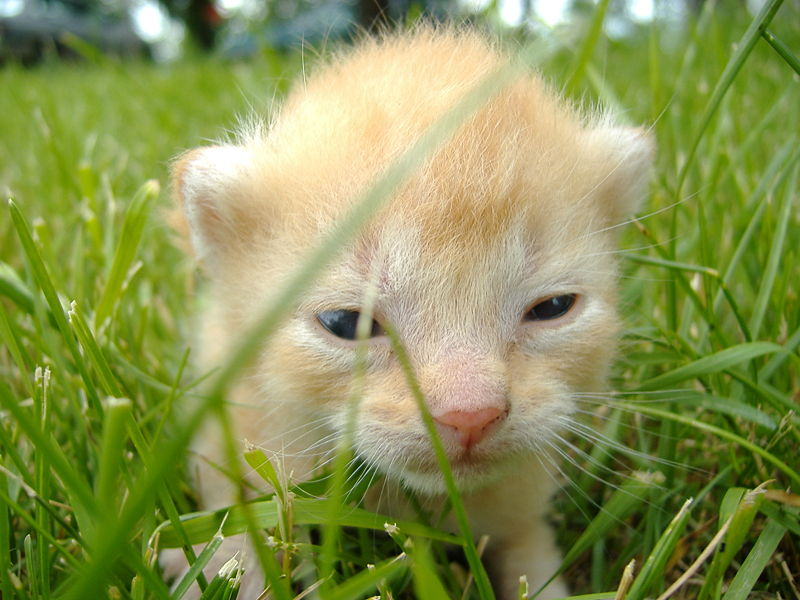
\includegraphics[width=.9\textwidth]{youngkitten}
    \caption{\LARGE Я прозрел!}
  \end{figure}
\end{frame}


%%%

\subsection{Что такое ``система управления версиями''?}

\begin{frame}{Что такое ``система управления версиями''?}
  \raisebox{-.30em}{\Large\HandRight}\hspace{.25em} Система управления
  версиями (англ. \emph{Version Control System}, сокр. \emph{VCS}) --
  ПО для облегчения работы с изменяющейся информацией. \vspace{1em}

  Основные возможности систем управления версиями:
  \begin{itemize}
  \item \alert{Обратимость} -- возможность вернуться к предыдущему
    состоянию.
  \item \alert{Согласованность} -- возможность совместной работы с
    одними и теми же данными в одно и то же время.
  \item \alert{Аннотирование} -- возможность сохранять метаданные об
    изменениях, комментарии от автора изменений.
  \end{itemize}

  \medskip

  Базовые операции:
  \begin{itemize}
  \item Получение рабочей копии файлов из репозитория.
  \item Запись изменений в репозиторий.
  \item Просмотр истории файлов.
  \end{itemize}
\end{frame}


%%%

\subsection{Области использования VCS}

\begin{frame}{Области использования VCS}
  Как самостоятельное приложение:
  \begin{itemize}
  \item Разработка ПО.
  \item Web-разработка.
  \item Научные работы, книги, ...
  \item Векторная графика.
  \item Хранение конфигурационных файлов.
  \item ...
  \end{itemize}
  В составе других приложений:
  \begin{itemize}
  \item Wikipedia и другие wiki.
  \item Системы документооборота (например, Alfresco.)
  \item ``Облачные'' сервисы (Google Docs, файловые хранилища.)
  \item Текстовые процессоры.
  \item ...
  \end{itemize}
\end{frame}


%%%

\subsection{Общая терминология}

\begin{frame}{Общая терминология}
  \begin{itemize}
  \item Репозиторий (англ. \emph{repository})
  \item ``Чекаут'' (англ. \emph{check out}, сокр. \emph{co})
  \item Рабочая копия (англ. \emph{working copy})
  \item Различие (англ. \emph{change}, \emph{diff}, \emph{delta})
  \item Коммит, ``чек-ин'' (англ. \emph{commit}, \emph{check-in},
    сокр. \emph{ci})
  \item Коммиттер (англ. \emph{committer})
  \item Ветвь (англ. \emph{branch})
  \item Ветвление (англ. \emph{branching})
  \item Верхушка, или ``голова'' ветви (англ. \emph{tip}, \emph{head})
  \item Слияние, мёрж (англ. \emph{merge})
  \item Конфликт (англ. \emph{conflict}, \emph{merge conflict})
  \item Метка, тэг (англ. \emph{label}, \emph{tag})
  \end{itemize}
\end{frame}


%%%

\subsection{Виды систем управления версиями}

\begin{frame}{Классификация систем управления версиями -- 1}
  \begin{figure}[htb]
    \centering
    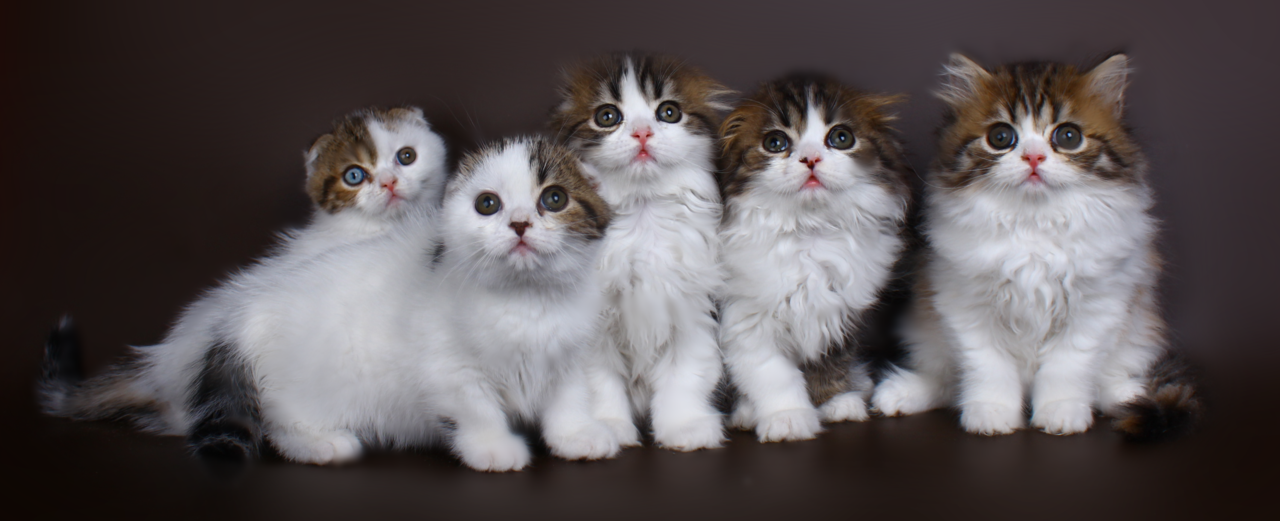
\includegraphics[width=.9\textwidth]{scottish-kitten}
  \end{figure}

  По расположению репозитория:
  \begin{itemize}
  \item \alert{Локальные} системы управления версиями (Local VCS)
  \item \alert{Централизованные} (клиент-серверные) системы управления
    версиями (Centralized VCS)
  \item \alert{Распределённые} системы управления версиями (Distributed VCS)
  \end{itemize}
\end{frame}

\begin{frame}{Классификация систем управления версиями -- 2}
  По способу работы с файлами:
  \begin{itemize}
  \item Оперирующие отдельными файлами
  \item Оперирующие наборами файлов
  \end{itemize}

  \medskip

  По способу разрешения конфликтов:
  \begin{itemize}
  \item Блокировка
  \item Слияние изменений
    \begin{itemize}
    \item Перед коммитом
    \item После коммита
    \end{itemize}
  \end{itemize}

  \medskip

  По способу сохранения истории:
  \begin{itemize}
  \item Различия между версиями (дельты)
  \item Слепки состояния (снэпшоты)
  \end{itemize}

  \ldots
\end{frame}


%%%

\subsection{История систем управления версиями}

\begin{frame}{История систем управления версиями}
  \begin{figure}[htb]
    \centering
    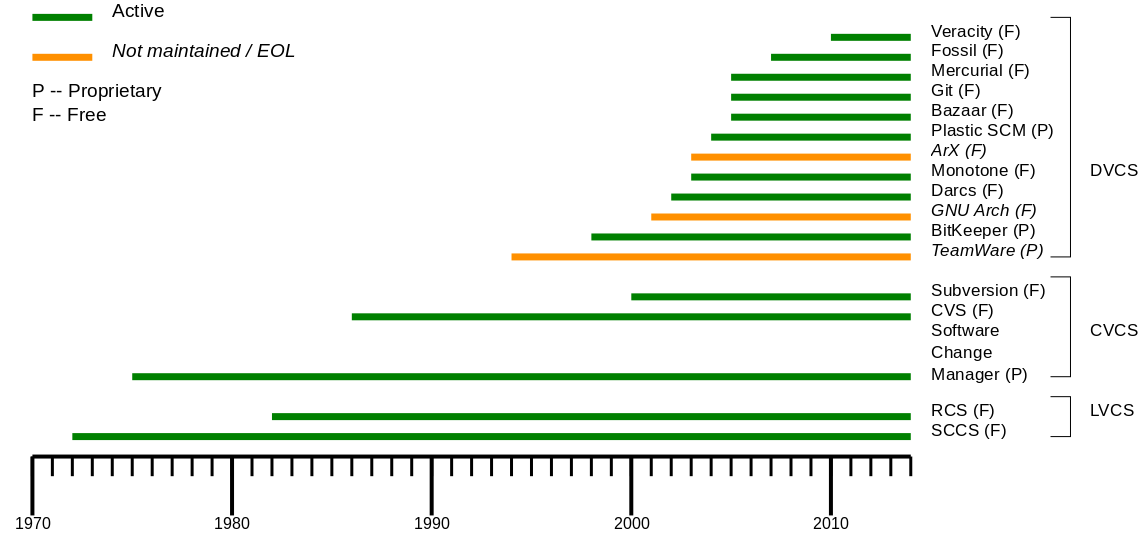
\includegraphics[width=1.05\textwidth]{vcs-timeline}
  \end{figure}
\end{frame}


%%%

\subsection{Вопрос выбора}

\begin{frame}{Вопрос выбора}
  \begin{figure}[htb]
    \centering
    
\includegraphics[width=.7\textwidth]{scurred}
    \caption{\Large Какую VCS выбрать?}
  \end{figure}
\end{frame}


%%%

\subsection{Локальные системы управления версиями}

\begin{frame}{Локальные системы управления версиями}
  \begin{figure}[htb]
    \centering 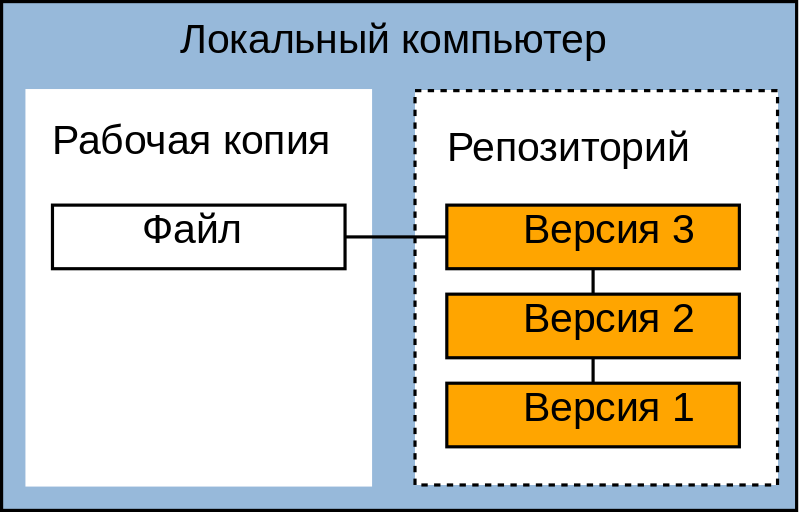
\includegraphics[width=1.0\textwidth]{vcs-local}
  \end{figure}
\end{frame}

\begin{frame}{Revision Control System (RCS)}
  Сайт: \url{gnu.org/s/rcs}\newline
  Некоторые факты:
  \begin{itemize}
  \item Создана примерно в 1982-м году.
  \item Локальная, оперирует отдельными файлами, использует блокировку
    для предотвращения конфликтов.
  \end{itemize}

  Преимущества:
  \begin{itemize}
  \item Проста в использовании.
  \end{itemize}

  Недостатки:
  \begin{itemize}
  \item Работа с ветками может быть нетривиальной.
  \item Каждый файл отслеживается отдельно.
  \item Не предоставляет контроль целостности.
  \item Не позволяет удалять файлы.
  \item Нет поддержки переименования файлов.
  \item Нет поддержки проектов с несколькими каталогами.
  \item \ldots{}
  \end{itemize}
\end{frame}


\begin{frame}[fragile]{Пример использования RCS}
  \begin{enumerate}
    \item Переходим в каталог с проектом: \newline
      \texttt{\$ cd \char`~/src/my-project}
    \item Создаём служебный каталог RCS: \newline
      \texttt{\$ mkdir RCS}
    \item "Чекиним" (коммитим) новый файл: \newline
      \texttt{\$ ci hello-world.txt}
      \newline
      При чекине RCS предложит ввести описание коммита.
    \item "Чекаутим" файл, с блокировкой для редактирования: \newline
      \texttt{\$ co -l hello-world.txt}
    \item Редактируем файл \ldots
    \item Чекиним изменения: \newline
      \texttt{\$ ci -l hello-world.txt}
    \item Смотрим лог: \newline
      \texttt{\$ rlog hello-world.txt}
  \end{enumerate}
\end{frame}


%%%

\subsection{Централизованные системы управления версиями}

\begin{frame}{Централизованные системы управления версиями}
  \begin{figure}[htb]
    \centering 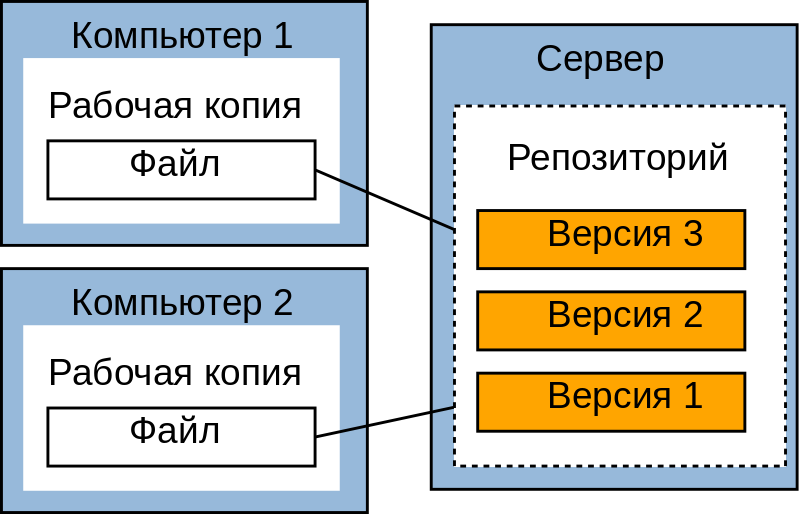
\includegraphics[width=1.0\textwidth]{vcs-centralized}
  \end{figure}
\end{frame}

\begin{frame}{Subversion (SVN)}
  Сайт: \url{subversion.apache.org}\newline
  Некоторые факты:
  \begin{itemize}
    \item Создана в 2000-м году.
    \item Централизованная, оперирует наборами файлов, использует
      слияние изменений для разрешения конфликтов.
  \end{itemize}
  Преимущества:
  \begin{itemize}
    \item Атомарные коммиты.
    \item Возможность переименования, копирования, перемещения и удаления
      файлов с сохранением истории.
    \item Работа с каталогами, символическими ссылками.
    \item Поддержка бинарных файлов.
    \item Позволяет легко увидеть общую картину -- кто и над чем
      работает.
    \item Предоставляет администратору полный контроль над доступом к
      репозиторию.
  \end{itemize}  
\end{frame}


\begin{frame}{Централизованные VCS ограничивают вашу свободу!}
  \begin{columns}
    \begin{column}{0.5\textwidth}
      \begin{figure}[htb]
        \centering
        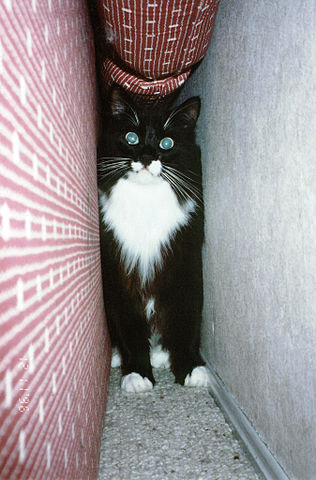
\includegraphics[width=.8\textwidth]{cat-hiding}
        \caption{В нашем проекте используют централизованную VCS.}
      \end{figure}
    \end{column}
    \begin{column}{0.5\textwidth}
      \begin{figure}[htb]
        \centering
        
\includegraphics[width=.8\textwidth]{packing-for-a-trip}
        \caption{В нашем проекте используют ClearCase.}
      \end{figure}
    \end{column}
  \end{columns}
\end{frame}


\subsubsection{Недостатки централизованных VCS}

\begin{frame}{Недостатки централизованных VCS}
  \begin{itemize}
  \item В случае недоступности сервера вы ограничены в действиях.
  \item Скорость выполнения операций зависит от скорости подключения к
    серверу.
  \item Единая точка отказа.
  \item Централизация диктует способ организации работы команды.
  \end{itemize}
\end{frame}


%%%

\subsection{Распределённые системы управления версиями}

\begin{frame}{Распределённые системы управления версиями}
  \begin{figure}[htb]
    \centering
    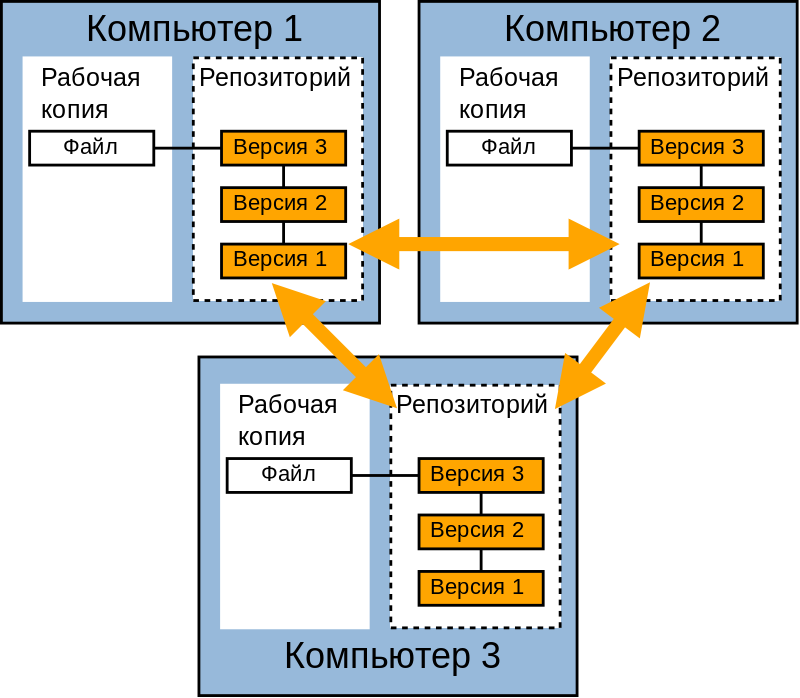
\includegraphics[height=.9\textheight]{vcs-decentralized}
  \end{figure}
\end{frame}

\begin{frame}{Преимущeства распределённых VCS}
  \begin{itemize}
  \item Нет зависимости от одного сервера, каждый клон является
    полноценным репозиторием $\Rightarrow$ нет единой точки отказа
  \item Большая часть операций локальны $\Rightarrow$ высокая скорость
    работы, нет зависимости от подключения к сети
  \item Взаимодействие между разработчиками организовано по принципу
    peer-to-peer $\Rightarrow$ возможна адаптация различных моделей
    разработки
  \item Не нужно поднимать сервер $\Rightarrow$ проще начать работу
  \end{itemize}
  \medskip
  \centering
  \LARGE Все преимущества локальных VCS плюс дополнительные ``плюшки''
  современных VCS.  Бесплатно!
\end{frame}

\begin{frame}{Вау!}
      \begin{figure}[htb]
        \centering
        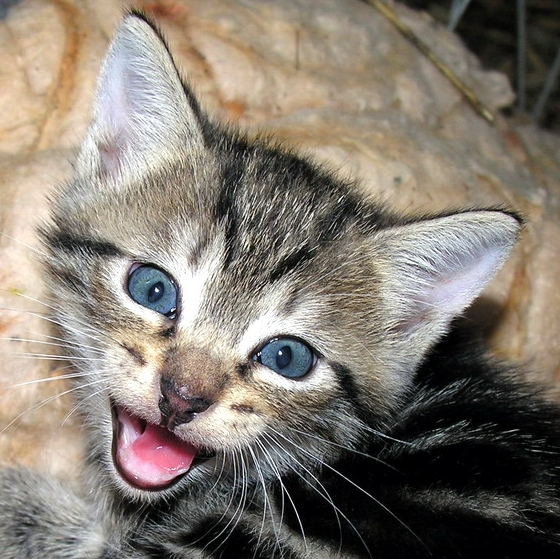
\includegraphics[width=.8\textheight]{kitty-meowing}
        \caption{\LARGE Вау!}
      \end{figure}
\end{frame}


%%%

\section{Cистема управления версиями Git}

\subsection{И тут на сцену выходит Git}

\begin{frame}{И тут на сцену выходит Git}
  \begin{figure}[htb]
    \centering 
\includegraphics[width=.6\textheight]{Git-logo}
  \end{figure}
  \vspace{-5pt}
  \begin{itemize}
  \item Сайт: \url{git-scm.com}
  \item Создан в 2005-м году; история Git связана с историей ядра Linux.
  \item Распределённый, оперирует наборами файлов, хранит слепки
    состояния.
  \item Следит за целостностью данных.
  \item Большая часть операций локальны.
  \item Поддержка нелинейной разработки, лёгкость создания веток и
    работы с ними.
  \item Возможность использования различных моделей организации работы
    команды.
  \item Эффективная работа с большими проектами.
  \end{itemize}
\end{frame}


%%%

\subsection{Терминология Git}

\begin{frame}{Терминология Git}
  \begin{figure}[htb]
    \centering
    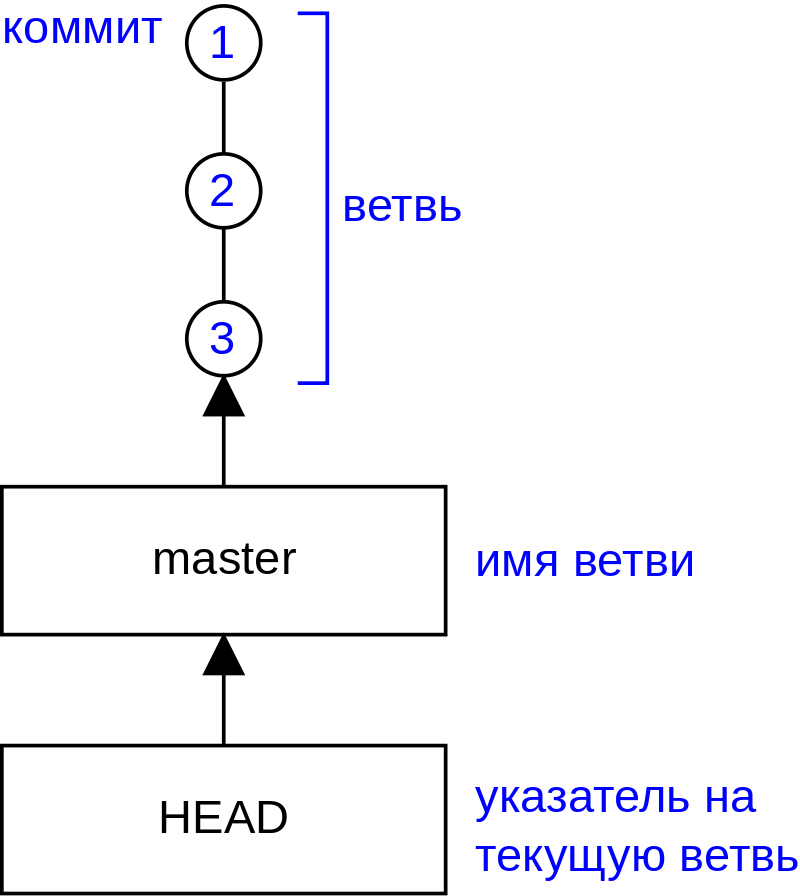
\includegraphics[height=.9\textheight]{git-basics-0}
  \end{figure}
\end{frame}

\subsection{Локальные операции}

\begin{frame}{Локальные операции}
  \begin{figure}[htb]
    \centering
    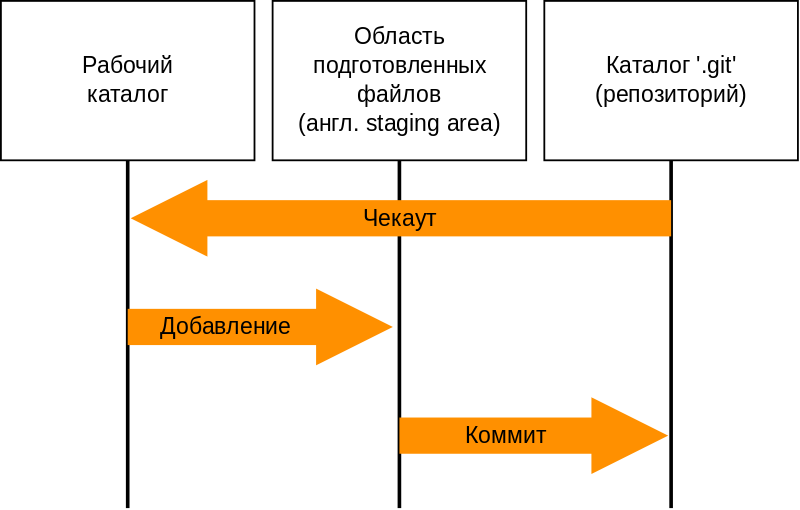
\includegraphics[width=1\textwidth]{git-local-operations}
  \end{figure}
\end{frame}


%%%

\subsection{Начало работы с Git}

\begin{frame}[fragile]{Начало работы с Git}
  \textbf{Задаём основные настройки:}
\begin{verbatim}
$ git config --global user.name  "Vasily I. Pupkin"
$ git config --global user.email "vip@example.ru"
\end{verbatim}
  \textbf{Смотрим пользовательский файл настроек:}
\begin{verbatim}
$ cat ~/.gitconfig
[user]
        name  = Vasily I. Pupkin
        email = vip@example.ru
\end{verbatim}
  \textbf{Получение справки:}
\begin{verbatim}
$ git --help         # Список часто используемых команд
$ git config -h      # Краткая справка
$ git config --help  # Подробная справка (man-страница)
$ man git-config     # man-страница команды
\end{verbatim}
\end{frame}

\begin{frame}[fragile]{Базовые команды}
  \begin{enumerate}
  \item Переходим в каталог с проектом: \newline
    \texttt{\$ cd \char`~/src/my-project}
  \item Инициализируем репозиторий: \newline
    \texttt{\$ git init}
  \item Подготавливаем файл к коммиту: \newline
    \texttt{\$ git add hello-world.txt}
  \item Коммитим изменения: \newline
    \texttt{\$ git commit -m "Initial commit"}
  \item Меняем файл \texttt{hello-world.txt} \ldots
  \item Подготавливаем изменения к коммиту: \newline
    \texttt{\$ git add hello-world.txt}
  \item Коммитим изменения: \newline
    \texttt{\$ git commit -m "hello-world.txt: Update"}
  \item Смотрим историю изменений: \newline
    \texttt{\$ git log}
  \end{enumerate}
\end{frame}


%%%

\subsection{Подробнее об основных командах}


%%%

\subsubsection{git init}

\begin{frame}[fragile]{\texttt{git init}}
  \textbf{Начальное состояние каталога с проектом:}
\begin{verbatim}
$ cd ~/src/my-project/
$ ls -A
hello-world.txt
$ cat hello-world.txt
hello
\end{verbatim}

  \textbf{Инициализируем пустой репозиторий:}
\begin{verbatim}
$ git init
Инициализирован пустой репозиторий Git
в /home/vip/src/my-project/.git/
\end{verbatim}

  \textbf{Что в каталоге?}
\begin{verbatim}
$ ls -A
.git  hello-world.txt
\end{verbatim}
\end{frame}


%%%

\subsubsection{git status}

\begin{frame}[fragile]{\texttt{git status}}
  \textbf{Смотрим, что получилось:}
\begin{verbatim}
$ git status
На ветке master

Начальный коммит

Неотслеживаемые файлы:
  (используйте «git add <файл>…», чтобы добавить в то,
   что будет включено в коммит)

	hello-world.txt

ничего не добавлено в коммит, но есть неотслеживаемые
файлы (используйте "git add", чтобы отслеживать их)
\end{verbatim}
\end{frame}


%%%

\subsubsection{git add}

\begin{frame}[fragile]{\texttt{git add}}
  \begin{columns}
    \begin{column}{0.6\textwidth}
  \textbf{Добавляем новый файл:}
\begin{verbatim}
$ git add hello-world.txt
\end{verbatim}
  \textbf{Смотрим на результат:}
\begin{verbatim}
$ git status
На ветке master

Начальный коммит

Изменения, которые будут
включены в коммит:
  (используйте 
   «git rm --cached <файл>…»,
   чтобы убрать из индекса)

	новый файл:    hello-world.txt
\end{verbatim}
    \end{column}
    \begin{column}{0.4\textwidth}
      \begin{figure}[htb]
        \centering
        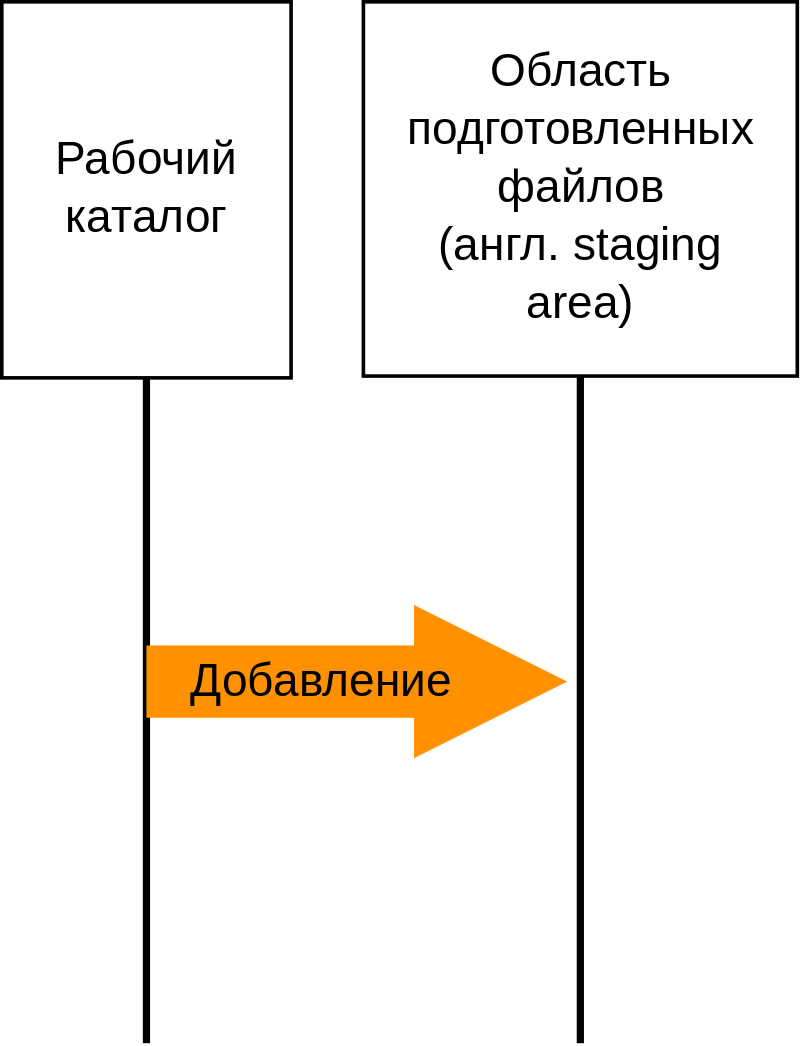
\includegraphics[width=1\textwidth]{git-operation-add}
      \end{figure}
    \end{column}
  \end{columns}
\end{frame}


%%%

\subsubsection{git commit}

\begin{frame}[fragile]{\texttt{git commit}}
  \begin{columns}
    \begin{column}{0.6\textwidth}
      \textbf{Коммитим изменения:}
\begin{verbatim}
$ git commit -m "Initial commit"
[master (корневой коммит) d4ef969]
    Initial commit
 1 file changed, 1 insertion(+)
 create mode 100644 hello-world.txt
\end{verbatim}
      \textbf{Смотрим на результат:}
\begin{verbatim}
$ git status
На ветке master
нечего коммитить, нет изменений
в рабочем каталоге
\end{verbatim}
  \textbf{Что в каталоге?}
\begin{verbatim}
$ ls -A
.git  hello-world.txt
\end{verbatim}
    \end{column}
    \begin{column}{0.4\textwidth}
      \begin{figure}[htb]
        \centering
        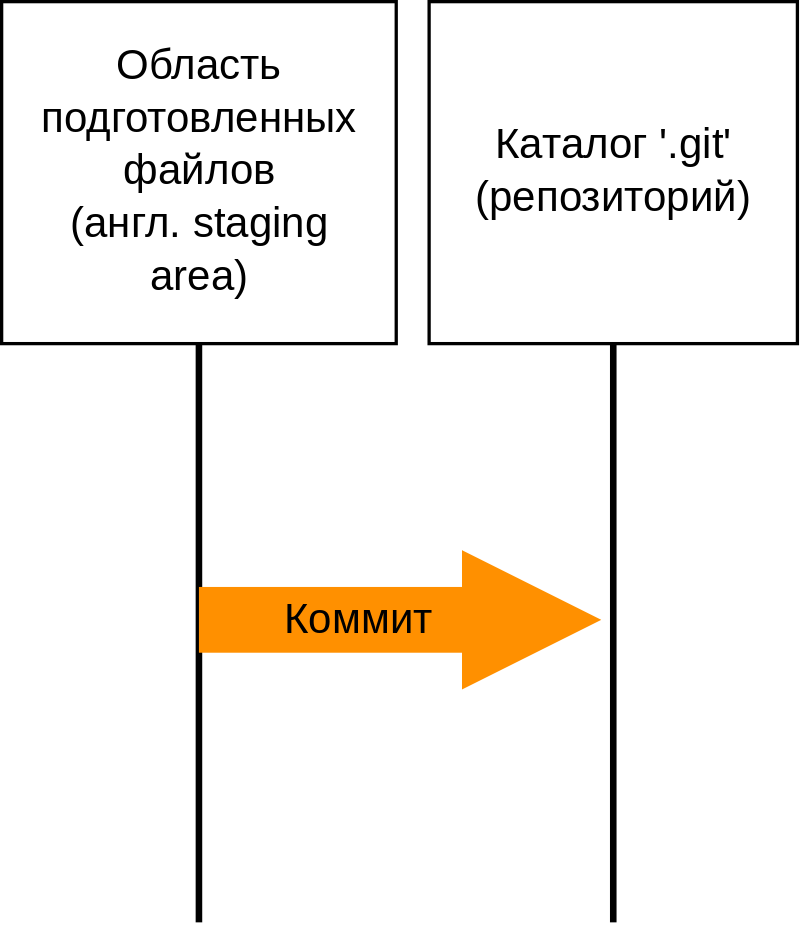
\includegraphics[width=1\textwidth]{git-operation-commit}
      \end{figure}
    \end{column}
  \end{columns}
\end{frame}


%%%

\subsubsection{git diff}

\begin{frame}[fragile]{\texttt{git diff} -- 1}
  \textbf{Делаем изменения:}
\begin{verbatim}
$ echo "world" >> hello-world.txt
\end{verbatim}
  \textbf{Смотрим различия:}
\begin{verbatim}
$ git diff
diff --git a/hello-world.txt b/hello-world.txt
index ce01362..94954ab 100644
--- a/hello-world.txt
+++ b/hello-world.txt
@@ -1 +1,2 @@
 hello
+world
\end{verbatim}
  \textbf{Коммитим изменения:}
\begin{verbatim}
$ git add hello-world.txt
$ git commit -m "hello-world.txt: Update"
\end{verbatim}
\end{frame}

\begin{frame}[fragile]{\texttt{git diff} -- 2}
  \begin{figure}[htb]
    \centering
    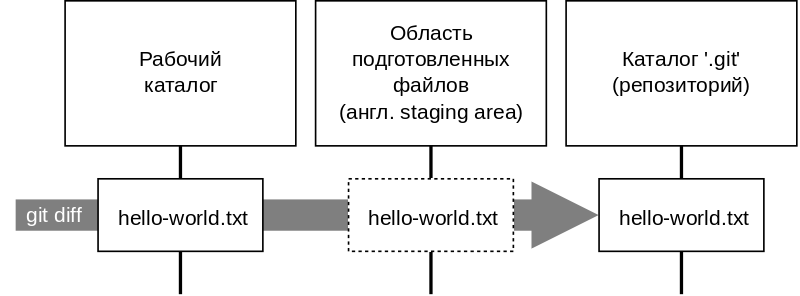
\includegraphics[width=1\textwidth]{git-operation-diff}
  \end{figure}
  \begin{itemize}
  \item Если файл \texttt{hello-world.txt} ещё не добавлен в область
    подготовленных файлов, то \texttt{git diff} сравнивает рабочую
    копию с версией из репозитория.
  \item Если \texttt{hello-world.txt} добавлен в область
    подготовленных файлов (через \texttt{git add}), то \texttt{git
      diff} сравнивает рабочую копию с подготовленной версией.
  \end{itemize}
\end{frame}


%%%

\subsubsection{git log}

\begin{frame}[fragile]{\texttt{git log}}
  \textbf{Смотрим лог изменений:}
\begin{verbatim}
$ git log
commit e3c28b5608ef0a2ab9f042d9633c4d6e1a5fc419
Author: Vasily I. Pupkin <vip@example.ru>
Date:   Sun Oct 18 11:57:55 2015 +0300

    hello-world.txt: Update

commit d4ef969a680fae0286b47ced166abfd6b7df30c1
Author: Vasily I. Pupkin <vip@example.ru>
Date:   Sun Oct 18 05:52:22 2015 +0300

    Initial commit
\end{verbatim}
\end{frame}

\begin{frame}{``Родословная'' коммитов}
  \begin{figure}[htb]
    \centering
    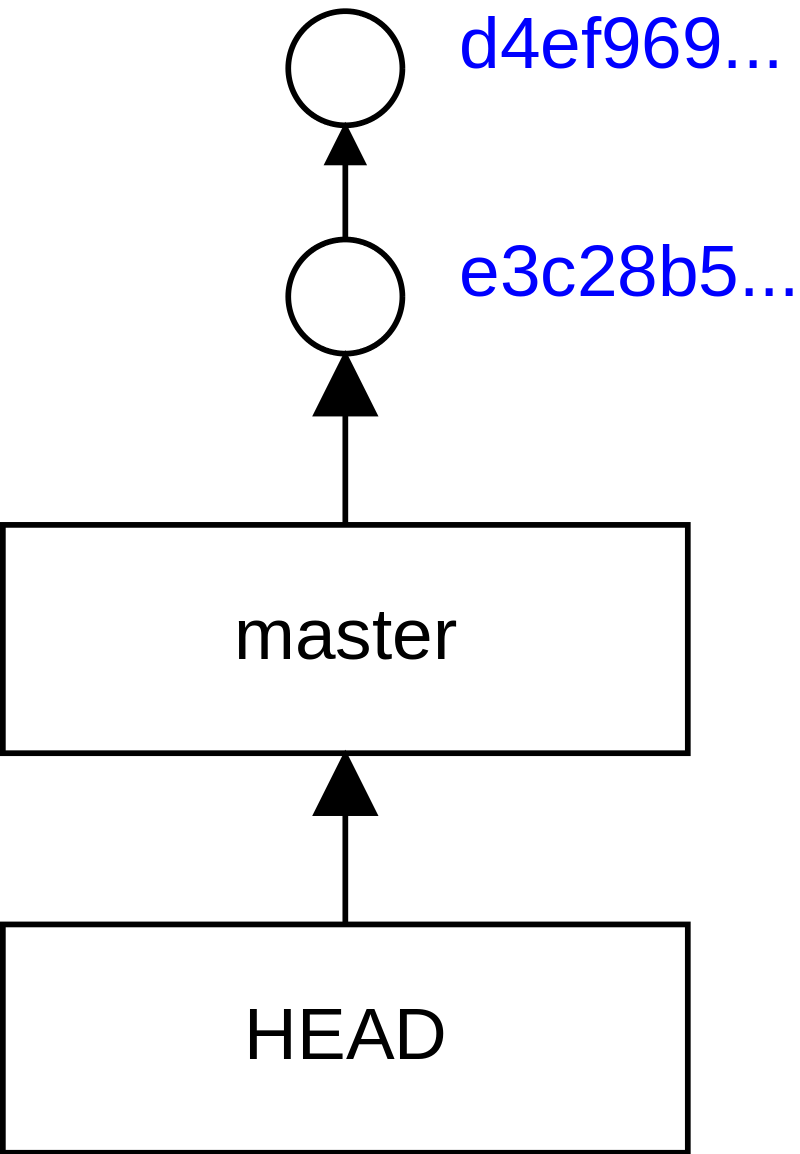
\includegraphics[height=.9\textheight]{git-basics-1}
  \end{figure}
\end{frame}

\begin{frame}{Что представляют из себя коммиты?}
  \center \LARGE Слепки состояния (англ. \emph{snapshots})
  \begin{figure}[htb]
    \centering
    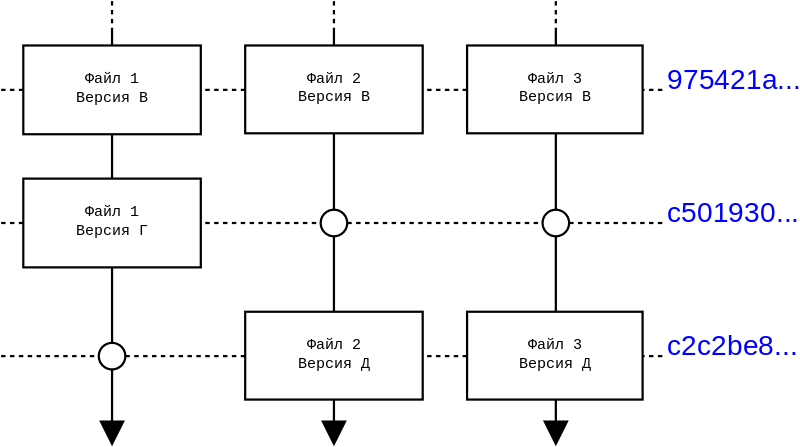
\includegraphics[width=.8\textwidth]{git-snapshots}
  \end{figure}
\end{frame}

\begin{frame}{И что?}
  \begin{figure}[htb]
    \centering
    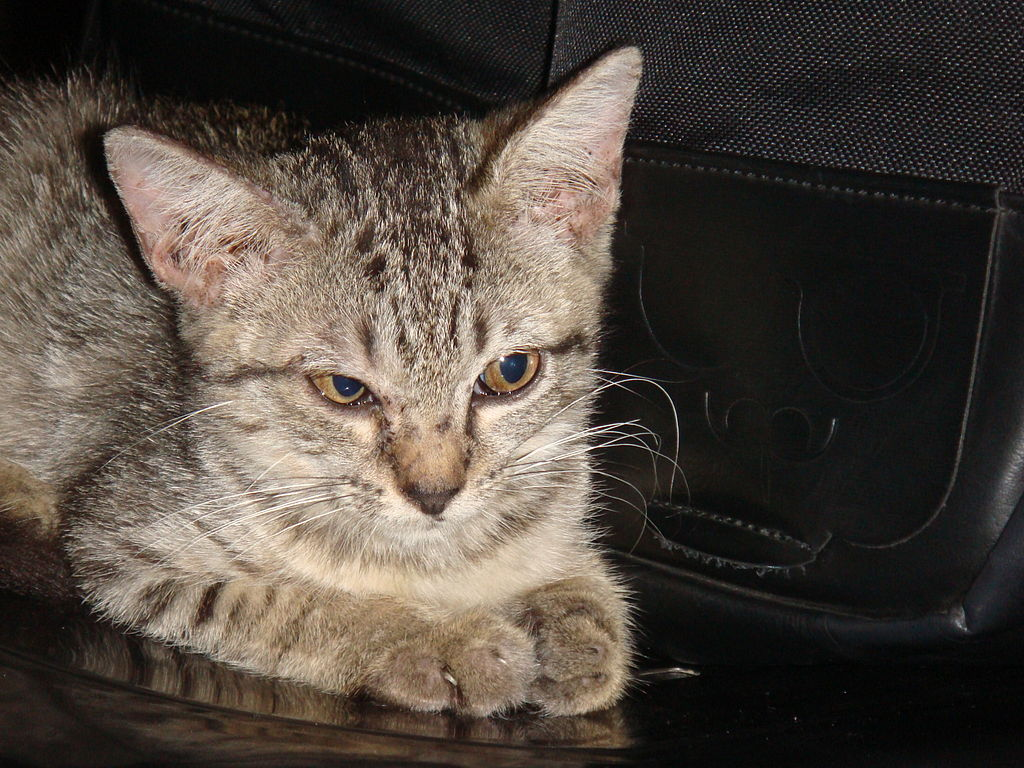
\includegraphics[width=.8\textwidth]{kucing-belang-perang}
    \caption{\LARGE Ну и зачем всё это?}
  \end{figure}
\end{frame}


%%%

\subsubsection{git checkout}

\begin{frame}[fragile]{\texttt{git checkout}}
  \centering
  \LARGE Ваша персональная машина времени!
  \normalsize
  \begin{columns}
    \begin{column}{0.6\textwidth}
\begin{verbatim}
$ cat hello-world.txt
hello
world
\end{verbatim}

  \textbf{Переключение на коммит:}
\begin{verbatim}
$ git checkout d4ef969
$ cat hello-world.txt
hello
\end{verbatim}

  \textbf{Переключение на ветвь \texttt{master}:}
\begin{verbatim}
$ git checkout master
$ cat hello-world.txt
hello
world
\end{verbatim}
    \end{column}
    \begin{column}{0.4\textwidth}
      \begin{figure}[htb]
        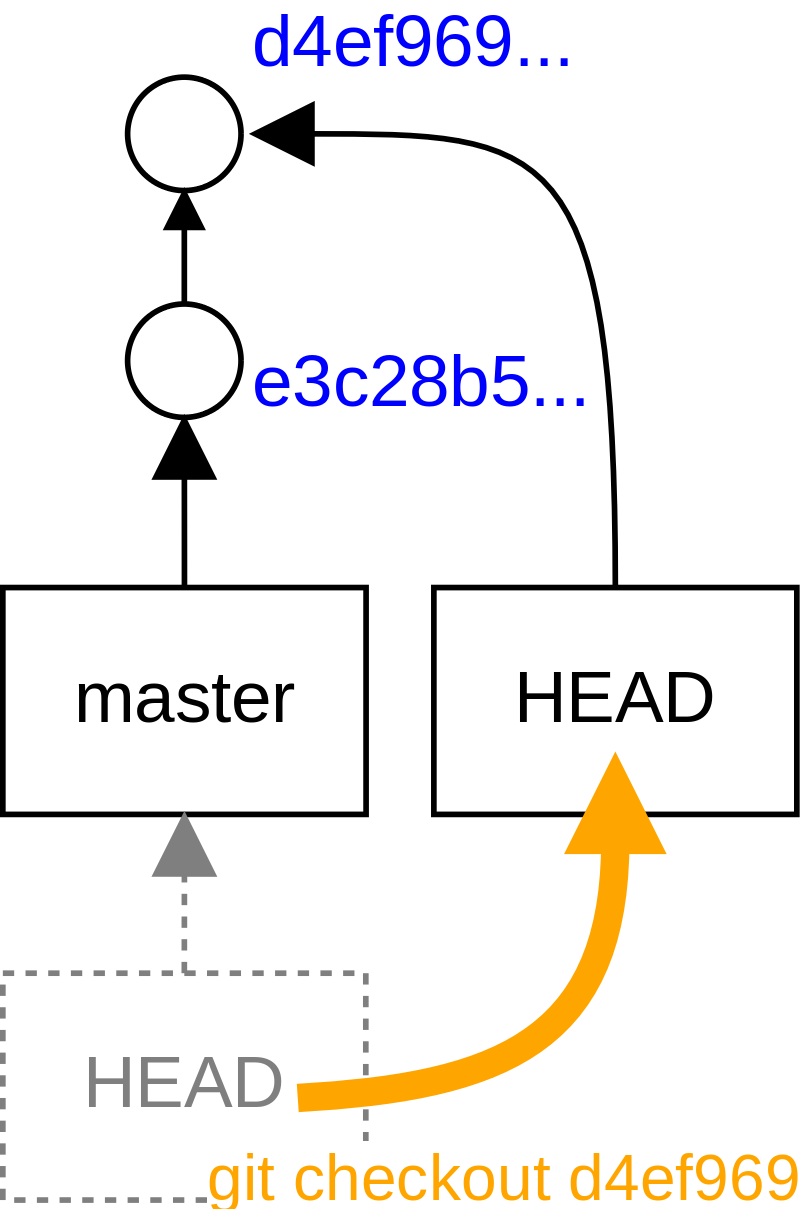
\includegraphics[width=1\textwidth]{git-operation-checkout}
      \end{figure}
    \end{column}
  \end{columns}
  \bigskip
\end{frame}


%%%

\subsection{Восстановление удалённых файлов}

\begin{frame}[fragile]{Восстановление удалённых файлов}
  \Large
  \textbf{Допустим, мы удалили важный файл:}
\begin{verbatim}
$ rm курсовая.tex
\end{verbatim}
\end{frame}

\begin{frame}[fragile]{Восстановление удалённых файлов}
  \begin{figure}[htb]
    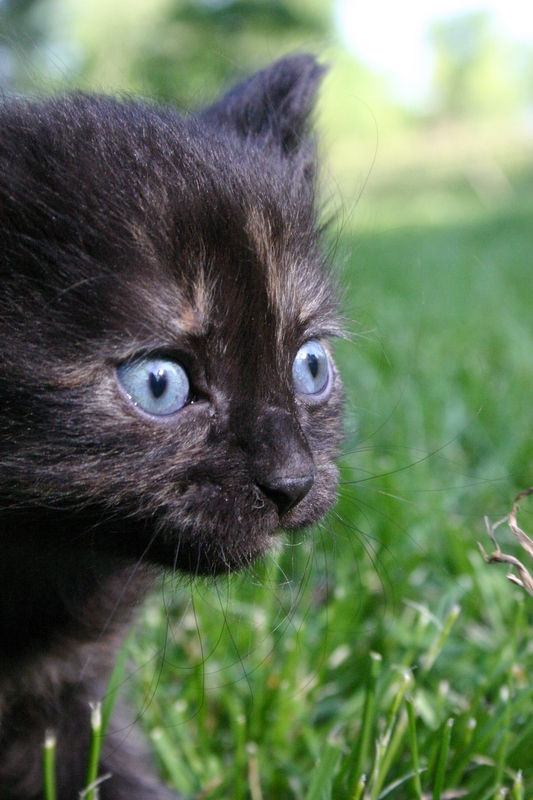
\includegraphics[height=.9\textheight]{blue-eyed-kitten}
  \end{figure}
\end{frame}

\begin{frame}[fragile]{Восстановление удалённых файлов}
  \Large
  \textbf{Допустим, мы удалили важный файл:}
\begin{verbatim}
$ rm курсовая.tex
\end{verbatim}
  \bigskip
  \textbf{Ой!..}\\[20pt]
  \textbf{Не беда, мы можем восстановить его из репозитория:}
\begin{verbatim}
$ git checkout курсовая.tex
\end{verbatim}
\end{frame}


%%%

\subsection{Операции над файлами}

\begin{frame}[fragile]{Операции над файлами}
  \textbf{Переименование и перемещение файлов:}
\begin{verbatim}
$ git mv hello-world.txt hello.txt
$ git status
На ветке master
Изменения, которые будут включены в коммит:
  (используйте «git reset HEAD <файл>…»,
     чтобы убрать из индекса)

  переименовано: hello-world.txt -> hello.txt
$ git commit -m "hello-world.txt: Rename"
\end{verbatim}

  \textbf{Удаление файлов:}
\begin{verbatim}
$ git rm hello-world.txt
$ git commit -m "hello-world.txt: Remove"
\end{verbatim}
\end{frame}


%%%

\subsection{Отмена операций}

\begin{frame}[fragile]{Отмена \texttt{git add} -- 1}
  \textbf{Добавляем изменения в область подготовленных файлов:}
\begin{verbatim}
$ git add hello-world.txt
$ git status
На ветке master
Изменения, которые будут включены в коммит:
  (используйте «git reset HEAD <файл>…»,
     чтобы убрать из индекса)

	изменено:      hello-world.txt
\end{verbatim}
  \textbf{Что делать, если мы поторопились?}
\end{frame}

\begin{frame}[fragile]{Отмена \texttt{git add} -- 2}
  \textbf{Удаляем файл из области подготовленных файлов:}
\begin{verbatim}
$ git reset hello-world.txt
$ git status
На ветке master
Изменения, которые не в индексе для коммита:
  (используйте «git add <файл>…», чтобы добавить файл
    в индекс)
  (используйте «git checkout -- <файл>…», чтобы 
    отменить изменения в рабочем каталоге)

	изменено:      hello-world.txt

нет изменений добавленных для коммита
(используйте «git add» и/или «git commit -a»)
\end{verbatim}
\end{frame}

\begin{frame}[fragile]{Отмена изменений в рабочем каталоге}
  \begin{columns}
    \begin{column}{0.6\textwidth}
  \alert{\textbf{Осторожно!  Здесь можно потерять незакоммиченные
      изменения!}}\newline\newline

  \textbf{Что делать, если мы сделали изменения, которые нам больше не
    нужны и мы не хотим их коммитить?  Отменить их!}
\begin{verbatim}
$ git checkout -- hello-world.txt
$ git status
На ветке master
нечего коммитить, нет изменений
в рабочем каталоге
\end{verbatim}
    \end{column}
    \begin{column}{0.4\textwidth}
      \begin{figure}[htb]
        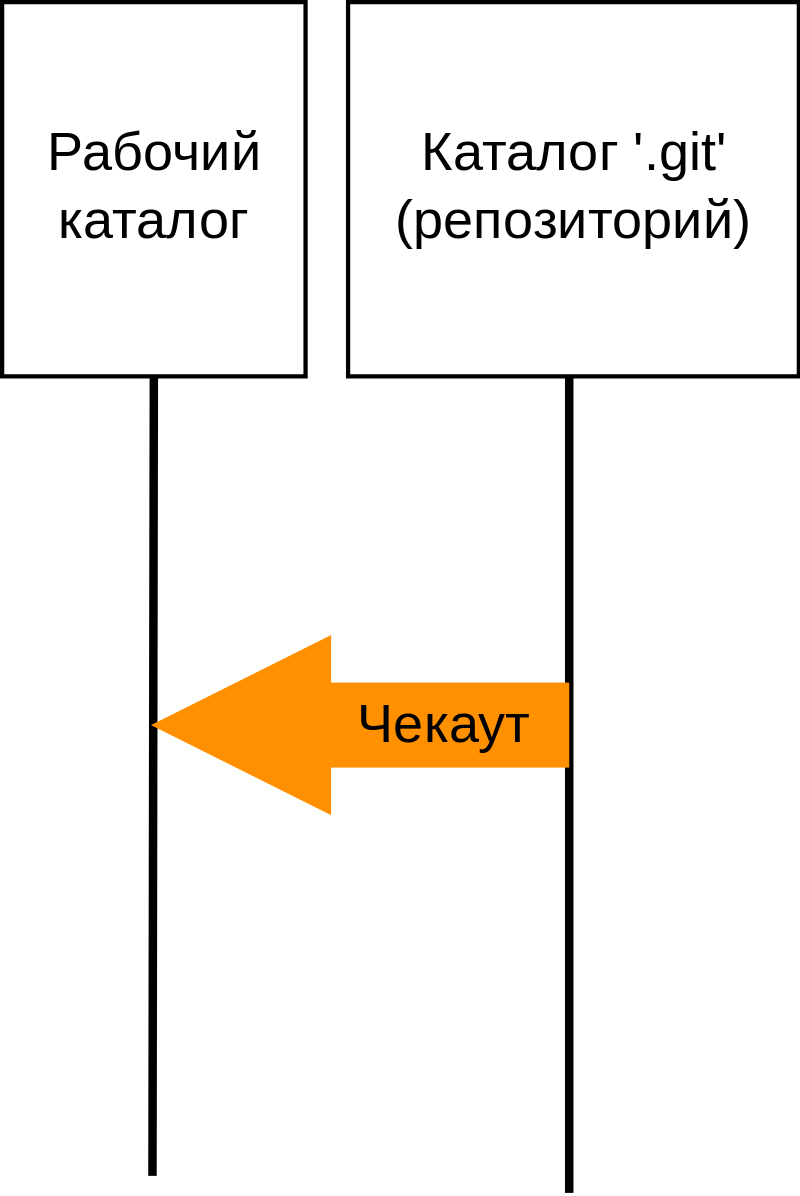
\includegraphics[width=1\textwidth]{git-operation-checkout-file}
      \end{figure}
    \end{column}
  \end{columns}
\end{frame}


%%%

\subsection{Клонирование репозитория}

\begin{frame}[fragile]{Клонирование репозитория}
  \textbf{Клонируем репозиторий:}
  \small
\begin{verbatim}
$ git clone \
    https://github.com/artyom-poptsov/talks.git \
    avp-talks
Клонирование в «avp-talks»…
remote: Counting objects: 161, done.
remote: Total 161 (delta 0), reused 0 (delta 0),
  pack-reused 161
Получение объектов: 100% (161/161), 18.19 MiB | 2.73 MiB/s,
  готово.
Определение изменений: 100% (48/48), готово.
Проверка соединения… готово.
\end{verbatim}
  \normalsize
  \textbf{Переходим в каталог с проектом:}
  \small
\begin{verbatim}
$ cd avp-talks
\end{verbatim}
\end{frame}


%%%

\section{Заключение}

\subsection{Заключение}

\begin{frame}{Заключение}

  Подробнее про Git на русском языке:
  \begin{itemize}
  \item Scott Chacon, Ben Straub, \textbf{``Pro Git''} --
    \url{https://www.git-scm.com/book/ru/v1}
  \item Александр Швец, \textbf{``Git How To: Курс обучения Git на
    русском''} -- \url{http://githowto.com/ru}
  \item Damir Shayhutdinov, \textbf{``Внутреннее устройство Git``} --
    \url{http://www.opennet.ru/base/dev/git\_guts.txt.html}
  \end{itemize}

  \bigskip

  Подробнее про системы управления версиями:
  \begin{itemize}
  \item Eric S. Raymond, \textbf{``Understanding Version-Control
    Systems''} --
    \url{http://www.catb.org/esr/writings/version-control/version-control.html}
  \item Rick Moen, \textbf{``Version-Control Systems for Linux''} --
    http://linuxmafia.com/faq/Apps/vcs.html
  \end{itemize}

\end{frame}

\subsection{Спасибо за внимание!}
\begin{frame}{Спасибо за внимание!}
  \large

  \raisebox{-.30em}{\Large\HandRight}\hspace{.25em} Ни один котёнок не
  пострадал при подготовке этой презентации! \\[30pt]

  Эл. почта: \url{poptsov.artyom@gmail.com}

  \medskip

  Презентация и её ``исходники'' под лицензией Creative Commons:
  \url{github.com/artyom-poptsov/talks/tree/master/vcs} \\[10pt]

  Спасибо, что выслушали  :-) \\[30pt]

  \bigskip

  \huge Вопросы?
\end{frame}


%%%

\begin{frame}{Использованные материалы}
  Фотографии котят и другие материалы c wikimedia.org:
  \begin{itemize}
  \item Dwight Sipler,
    \href{https://www.flickr.com/photos/photofarmer/411955683/}{``You
      know, I think the large trees are easier. (411955683)''} (CC-BY
    2.0)
  \item That Guy, From That Show!,
    \href{https://commons.wikimedia.org/wiki/File:Youngkitten.JPG}{``A
      kitten opens its eyes for the first time''} (PD)
  \item RN3DLL,
    \href{https://commons.wikimedia.org/wiki/File:Scottish_Kitten.png}{``Scottish
      Kitten''}, (CC-BY 3.0)
  \item ColKorn1982,
    \href{https://commons.wikimedia.org/wiki/File:Scurred.jpg}{``Coll
      little Orange Tabby kitten''} (CC-BY-SA 2.0)
  \item Dwight Sipler,
    \href{https://commons.wikimedia.org/wiki/File:Packing_for_a_trip_(302328043).jpg}{``Packing
      for a trip''} (CC-BY 2.0)
  \item Algerds,
    \href{https://commons.wikimedia.org/wiki/File:Kitty_meowing.jpg}{"Kitty
      meowing"} (CC-BY-SA 3.0)
  \item Pagedelete,
    \href{https://commons.wikimedia.org/wiki/File:Chizhik.jpg}{"Chizhik"}
    (CC-BY-SA 3.0)
  \item Karin Dalziel,
    \href{https://commons.wikimedia.org/wiki/File:Blue-eyed_kitten.jpg}{"Blue-eyed
      kitten"} (CC-BY 2.0)
  \item Kerina yin,
    \href{https://commons.wikimedia.org/wiki/File:Kucing_belang_perang_(brown_mackerel_tabby_cat).JPG}{``Kucing
      belang perang (brown mackerel tabby cat).''} (PD)
  \item Mysid, Incnis Mrsi,
    \href{https://commons.wikimedia.org/wiki/File:Computer_keyboard_US.svg}{"Computer
      keyboard US"} (PD)
  \item
    \href{https://commons.wikimedia.org/wiki/File:Git-logo.svg}{"Git
      logo"} (CC-BY 3.0)
  \end{itemize}

  \bigskip
\end{frame}

\begin{frame}{Лицензия}
  Copyright \textcopyright 2015 Artyom V. Poptsov
  <poptsov.artyom@gmail.com> \newline

  Права на копирование других изображений, использованных в данной
  работе, принадлежат их владельцам. \newline

  Данная работа распространяется на условиях лицензии Creative Commons
  Attribution-ShareAlike 4.0 International:
  \url{https://creativecommons.org/licenses/by-sa/4.0/}
\end{frame}

\end{document}

%%% lection0.tex ends here.
